%  
%  This template was created in order to facilitate the Call for 
%  Papers process for "Encuentro Linux 2009" and modified to be
%  used by upcoming events.
%  
%  --------------------------------------------------------------
%
%  History
%
%  Version 1: (2009)  
%   - Author: Arturo A. Hoffstadt Urrutia <ahoffsta@inf.utfsm.cl>
%   - EL2009 version.
%  Version 2: (27/07/2010)
%   - Author: Miguel Angel Ruiz Manzano <mruiz@openminds.cl>
%   - EL2010 version.
%   - Licenced under GPL.
%  Version 2.1: (06/08/2010)
%   - Author: Miguel Angel Ruiz Manzano <mruiz@openminds.cl>
%   - License update. The previous one was not well defined.
%
%  --------------------------------------------------------------
%
%  This file is distributed under the terms and conditions of the 
%  Attribution-NonCommercial-ShareAlike 3.0 Unported license. For
%  more information, please visit the following URL
%  
%  http://creativecommons.org/licenses/by-nc-sa/3.0/
%
%

\documentclass[letterpaper,12pt]{article}

\usepackage[spanish]{babel}
\usepackage{graphicx}
\usepackage[utf8]{inputenc}
\usepackage{fullpage}
\usepackage{url}
\usepackage{multicol}
\usepackage{amsmath}

\makeatletter
\renewcommand{\paragraph}{\@startsection{paragraph}{4}{0ex}%
   {-3.25ex plus -1ex minus -0.2ex}%
   {1.5ex plus 0.2ex}%
   {\normalfont\normalsize\bfseries}}
\makeatother

\stepcounter{secnumdepth}
\stepcounter{tocdepth}

\title{Guía de supervivencia para \\ contribuir al OSS}
\author{Leo Soto M.\\ \url{leo.soto@gmail.com}}
\date{\today}

\begin{document}
\begin{minipage}{0.1in}
  
\includegraphics[width=1.2in]{images/logo.png}
\end{minipage}
\hfill
\begin{minipage}{6in}
  \maketitle
\end{minipage}
\hfill
\begin{minipage}{7in}
%cambiar por su logo
%  
\includegraphics[width=1.2in]{images/logo.png}
\end{minipage}
  \thispagestyle{empty}

\begin{abstract}

  Involucrarse en un proyecto open source no es tarea fácil. Dejando afuera los
  aspectos técnicos de cada proyecto, una dificultad adicional es entender la
  dinámica social, los códigos y las expectativas de la comunidad de desarrollo
  OSS. Esta charla mostrará las lecciones obtenidas por el autor en su camino
  como desarrollador participando en diversos proyectos open source.

\end{abstract}

\textbf{Palabras Claves:} Código Abierto, Linux, Creative Commons, OSS

\section*{Introducción}

Las reglas de la comunidad open source no están escritas en ningún manual
definitivo. Existen guías y fuentes mas importantes que otras, pero la forma en
que un desarrollador, tester, diseñador, traductor o cualquier otro miembro
activo de un proyecto pasa a formar parte del mismo no está escrita.

La razón es muy simple: No existe \emph{la} forma de hacerlo. Mas allá de variar
de proyecto en proyecto, consiste también en una combinación de costumbres
sociales que han evolucionado durante los años y que también \emph{cambia} con
los años.

\section*{Motivación}

Es en estas circunstancias cuando la experiencia toma un valor adicional. Porque
a través de la experiencia de quienes han aprendido ha relacionarse con la
comunidad open source es como otros pueden aprender, o al menos hacerse una idea
de como involucrarse en ella de manera más efectiva.

¿Pero qué quiere decir ``involucrarse de manera más efectiva''?

Para este trabajo, el foco está en dos puntos: (a) hacer que los primeros
contactos no sean frustrantes y (b) que los resultados sean relativamente
inmediatos (i.e, conseguir que las contribuciones sean aceptadas por los
proyectos en los que se desea colaborar)

El autor ha de reconocer humildemente que su introducción en el mundo del OSS no
fue particularmente efectiva, fallando ambos criterios. Sin embargo, y mediante
la aplicación sistemática (y no tan sistemática) de la prueba y error, sumada
quizás a algo de madurez personal y muy probablemente acompañada de uno o dos
golpes de suerte, el autor es hoy un miembro activo (y efectivo) en varios
proyectos open source.

Lamentablemente, llegar a este punto tomó bastante tiempo y, en
retrospectiva, el autor considera que de haber recibido ciertos \emph{hints}, su
introducción al mundo OSS hubiera sido mucho más efectiva. 

Cansado de esperar la invención (¡y masificación!) de una máquina del tiempo que
le permita corregir tamaña injusticia, por ahora el autor se conforma con
difundir dichos \emph{hints} en esta charla\footnote{Que por cierto fue expuesta
  con éxito en la FLISOL 2010}. El objetivo es que \emph{otros} puedan
involucrarse en el opensource de manera efectiva. Y tal vez incluso salvar a mas
de alguien que en lugar de rendirse tras la primera frustración, consiga
entender que detrás del aparentemente frío y huraño mundo del desarrollo
opensource existe suele existir una comunidad de personas tan amable como
cualquier otra.

\section*{Desarrollo del Tema}

En su calidad de charla más motivacional que técnica, el trabajo se centra en
historias, anécdotas y lecciones consideradas como claves por el autor. La idea
es evitar quedarse en lo abstracto y mostrar en concreto como los \emph{hints}
dados han aplicado en la práctica a proyectos reales. A continuación se
describen los puntos principales a tratar, los cuales son entremezclados con
historias y reflexiones que por razones de espacio no se pueden incluir en este
documento.

\subsubsection*{Preguntas inteligentes}

Uno de los primeros errores que uno puede cometer al interactuar con los
desarrolladores de un proyecto OSS, es hacer las preguntas equivocadas. No hay
nada de malo en hacer preguntas, siempre y cuando sean mas o menos inteligentes.

Afortunadamente, sí existe un excelente escrito al respecto, con el original
título de ``Cómo hacer preguntas de manera inteligente''
\cite{PreguntasInteligentes}. Del contenido de dicho artículo, se hará énfasis
en (a) intentar encontrar una respuesta \emph{antes de preguntar}, (b) ser
preciso e informativo \emph{al preguntar}, (c) interpretar lo que se lee
\emph{cuando se recibe una respuesta}, y (d) Cómo no reaccionar.

Con esto se pretende cubrir rápidamente el ``ciclo de vida'' de una pregunta,
sin repetir el contenido completo del artículo original pero sí dejando una idea
de su contenido para que los interesados puedan luego leer el texto completo.

\subsubsection*{Escogiendo una primera contribución}

Una excelente estrategia para empezar es contribuir algo (a) simple y (b) que
tenga utilidad para uno mismo. Lo primero aumenta las probabilidades de poder
implementar la contribución en cuestión y que la implementación sea correcta.Lo
segundo le agrega una motivación práctica que asegura que la contribución está
resolviendo un problema concreto y real. Además de que, en el caso que la
contribución sea rechazada, siempre seguirá siendo útil para uno.

\subsubsection*{Inglés}

Mejorar el inglés es una necesidad. De lo contrario uno se aisla en los pocos
proyectos donde uno se puede dar el lujo de hablar solamente en español. Sin
embargo, no es necesario tener un inglés británico perfecto. En realidad ni
siquiera es tan necesario hablarlo. Basta con entender el inglés escrito y ser
capaz de escribir decentemente.

\subsubsection*{Seguir el bug tracker}

Una forma de ir aprendiendo cada vez más de cómo funciona un software es seguir
el bug tracker y, aunque no se pueda aportar con código, reportar los errores
que se encuentren. Una vez que alguien los arregle se podrá mirar cómo fue
arreglado el problema, y se aprenderá del código. Y luego, cuando sea posible
adjuntar parches a los reportes, los desarrolladores del proyecto muy
probablemente tendrán una buena disposición con uno.

\subsubsection*{Identificar cuando se ha tenido éxito}

Es muy simple saber que las contribuciones han caído en tierra fértil. Basta
observar si, de parte de los desarrolladores del proyecto, se observan dos
cosas: entusiasmo y colaboración. Si es así, aún cuando la contribución no haya
sido aceptada a la primera, lo será más temprano que tarde.

\subsubsection*{Conclusiones}

El cierre de la charla está dedicado a recapitular las lecciones obtenidas a lo
largo de las historias y anécdotas. Lecciones que incluyen algunos de los puntos
principales tratados, como hacer cosas que le sirvan a uno mismo y el
perfeccionar el inglés. Y también lecciones de vida que van mas allá del open
source como cultivar la paciencia, aprender a seguir antes que liderar y siempre
ensayar, errar y aprender. Y lo más importante: Tener ``cuero de chancho''.

\begin{thebibliography}{}

 \bibitem{PreguntasInteligentes} Eric S Raymond,  \textit{Cómo hacer preguntas inteligentes}, \url{http://www.sindominio.net/ayuda/preguntas-inteligentes.html}
\end{thebibliography}

\newpage

\begin{description}
 \item[Área en la que se centra el trabajo:] Desarrollo de software
 \item[Nivel:] Básico
 \item[Enfoque de la presentación:] .\\
  \begin{itemize}
   \item Todos los puntos tratados en el desarrollo del tema.
   \item La actitud de ``cuero-de-chancho'' que es transversal a dichos puntos.
   \item Reflexiones intermedias, incluyendo:
     \begin{itemize}
     \item Las consecuencias de que el open source permita que el código de uno
       sea usado de formas que uno nunca imaginó.
     \item La relación entre crear un proyecto opensource y crear un movimiento.
     \end{itemize}
  \end{itemize}
\end{description}

\newpage

\appendix
\section{Acerca del Autor}

\begin{figure}[h]
\begin{minipage}{11.5cm}

\subsection{Reseña}

Leo Soto es Ingeniero Informático de la USACH, socio de Continuum y
desarrollador para Hashrocket Chile. Como parte de su experiencia en el mundo
OSS, es parte del del equipo de desarrollo de Jython desde el 2008, tras haber
participado en el Google Summer of Code de ese mismo año. También es colaborador
en Mongoid, un ODM para el lenguaje Ruby y MongoDB, una base de datos no
relacional.

Ha dictado charlas fuera del país en la DjangoCon 2008 realizada en el
GooglePlex en Mountain View, y en la PyCon 2009 en Chicago. En el medio nacional
ha participado como expositor en las FLISOL 2009 y 2010, Encuentro Linux 2008 y
2009 y en las Jornadas Regionales del Software Libre 2009.

\end{minipage}
\begin{minipage}{1.7in}
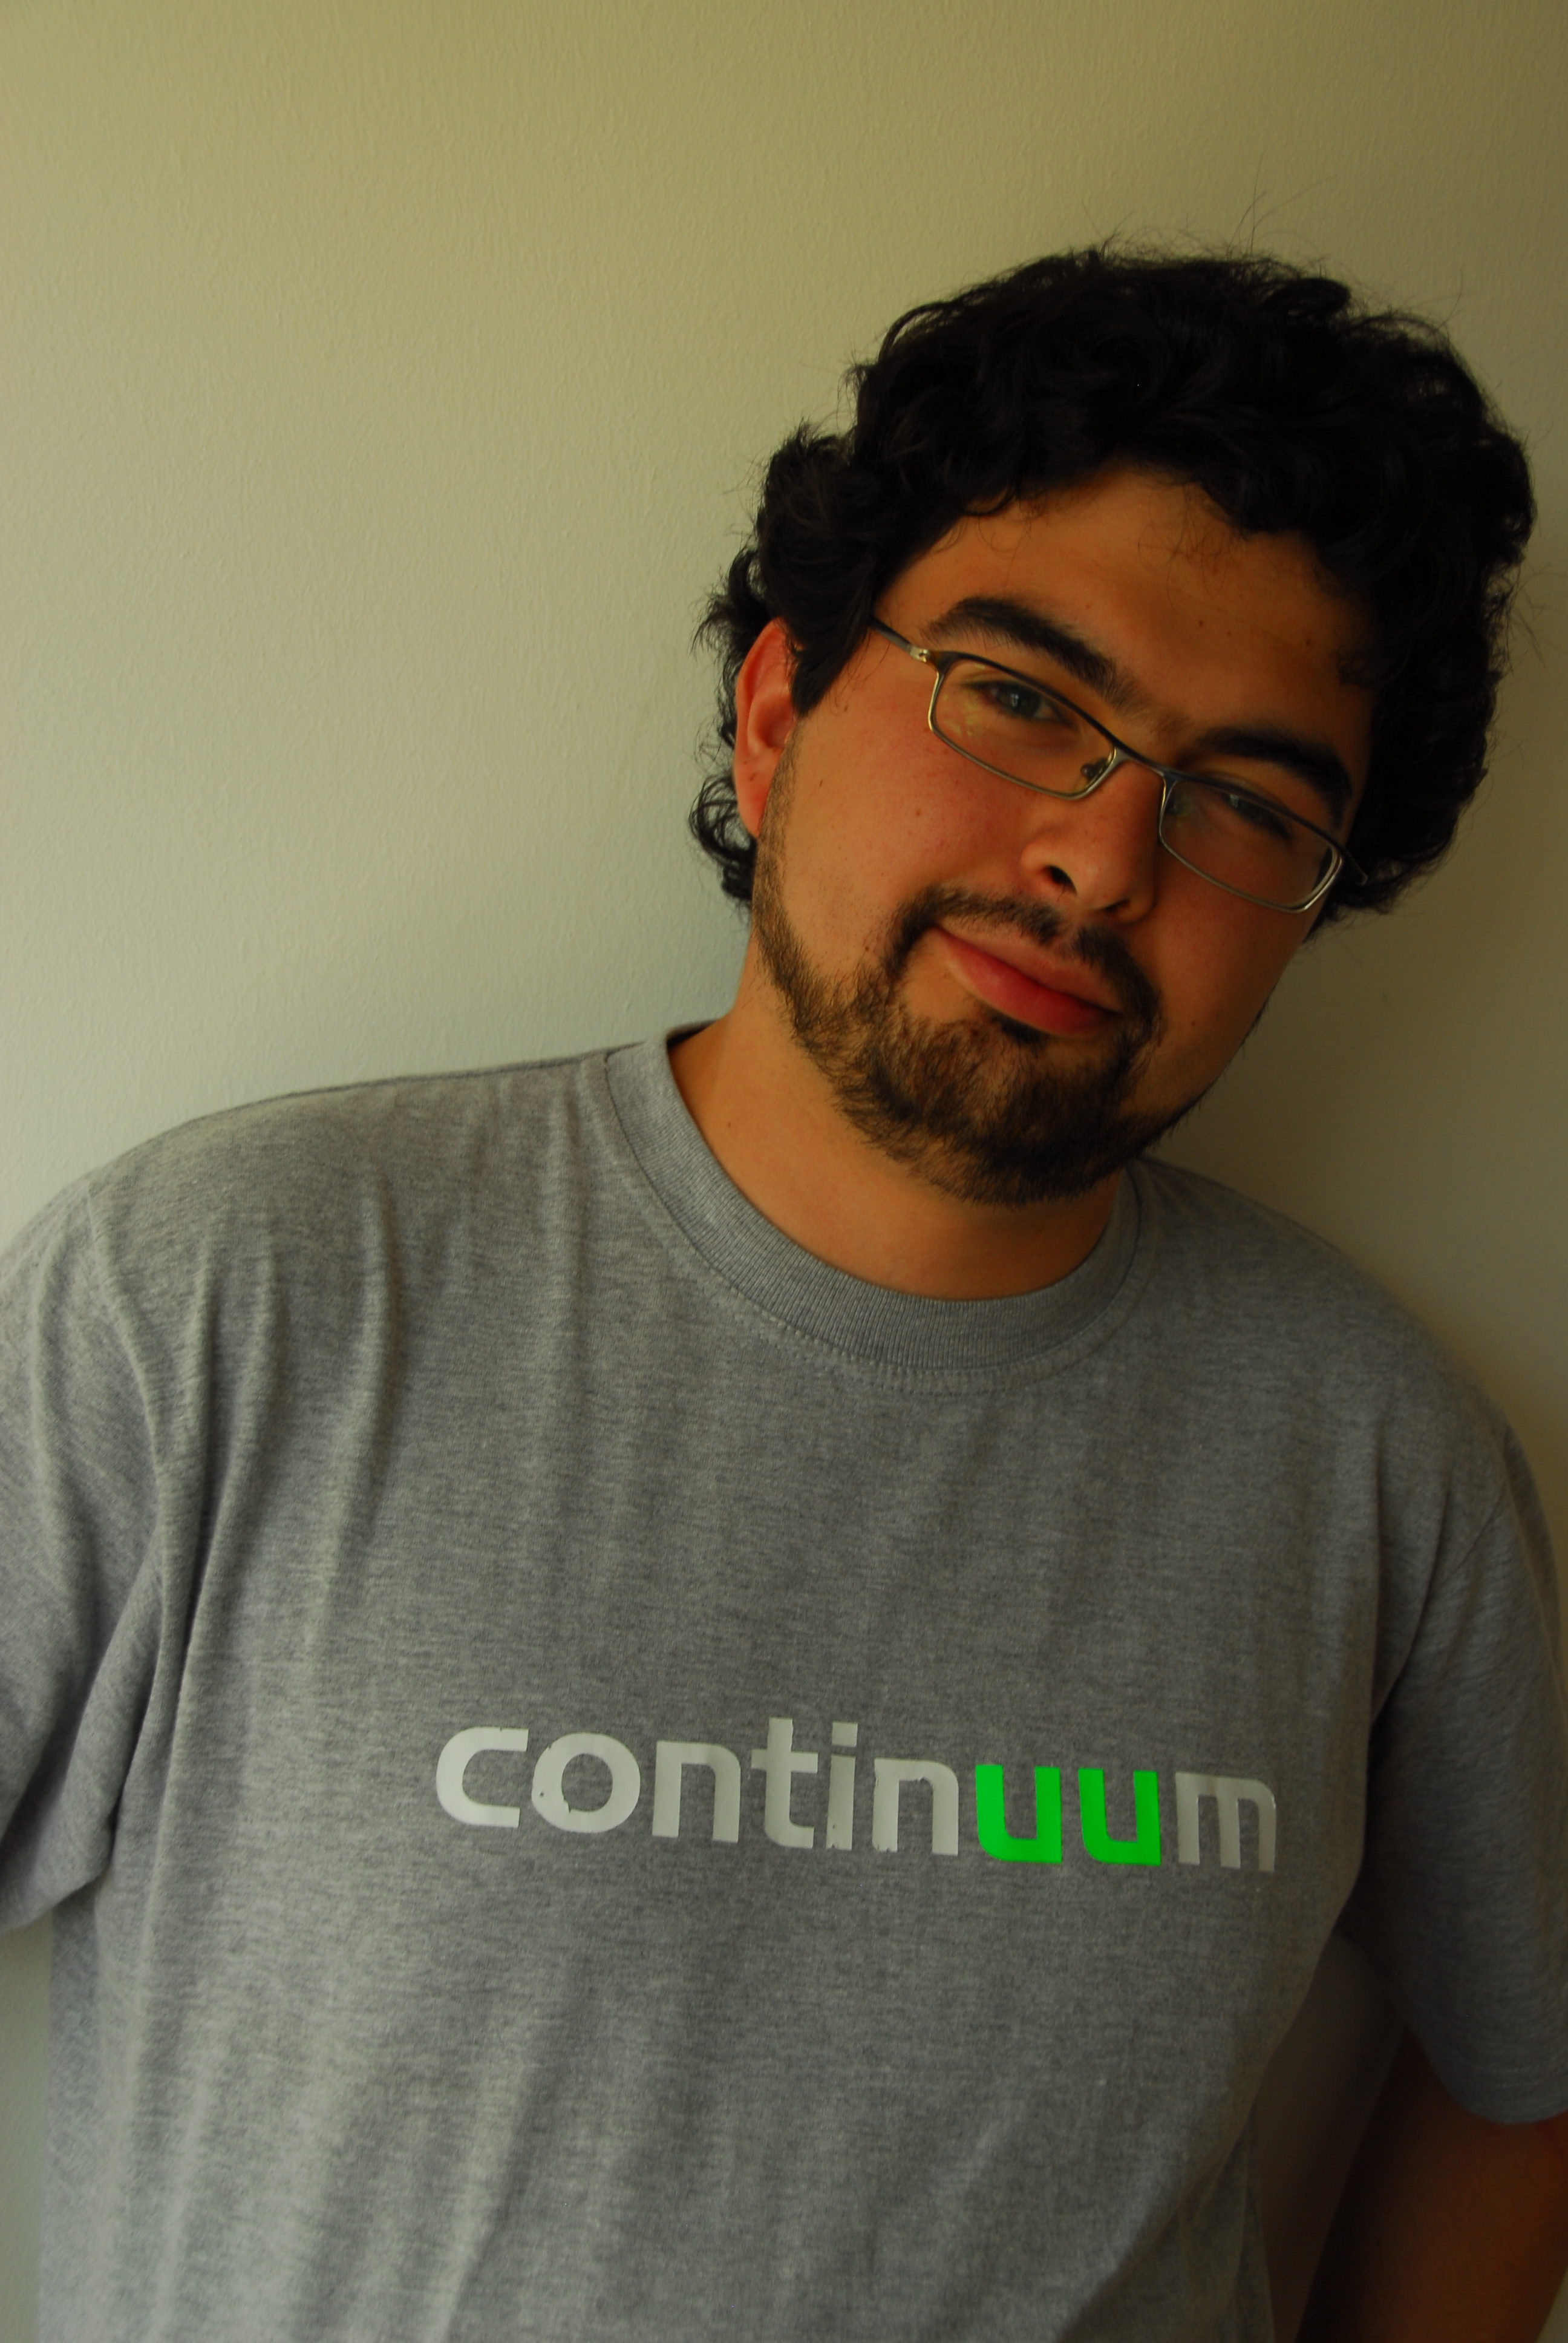
\includegraphics[width=1.5in]{images/DSC_0450.JPG}
\end{minipage}
\end{figure}

\subsection{Datos de contacto}

\begin{itemize}
\item{\textbf{E-mail:} leo.soto@gmail.com}
\item\textbf{{Teléfono:} 9 8733 9008}
\item{\textbf{URL:} \url{http://blog.leosoto.com}}
\end{itemize}


\end{document}
